\subsection{Informação Mútua}
\begin{frame}%[allowframebreaks]
  \frametitle{Intuição sobre Informação Mútua}
  \begin{itemize}
  \item Dadas duas variáveis aleatórias $X$ e $Y$, quanta informação uma possui sobre a outra?
  \item Conhecendo $X$, quanto sabemos sobre $Y$? Conhecendo $Y$, quanto sabemos sobre $X$?
  \item Se as v.a.s são independentes, $X \independent Y$, então conhecer $X$ não nos diz nada sobre
  $Y$ e vice-versa.
  \item Como temos uma medida de informação em uma fonte aleatória, $H(X)$, podemos quantificar
  quanta informação variáveis aleatórias possuem uma sobre as outras. Isto é chamado de 
  \underline{informação mútua}.
  \end{itemize}
\end{frame}

\begin{frame}%[allowframebreaks]
  \frametitle{Informação Mútua de Evento}
  Dado o evento $\{X=x, Y=y\}$, podemos nos perguntar sobre qual é a informação fornecida
  pelo evento $x$ dado o fato de que o evento $y$ ocorreu. Isto pode ser quantificado da seguinte forma:
  \begin{equation}
  I(x;y) = \log \frac{p(x|y)}{p(x)} = \underbrace{\log \frac{1}{p(x)}}_{A} - \underbrace{\log \frac{1}{p(x|y)}}_{B}
  \end{equation}
  
  \begin{itemize}
  \item Primeiro termo $A$: surpresa de que $x$ ocorreu.
  \item Segundo termo $B$: surpresa de que $x$ ocorreu dado que $y$ ocorreu.
  \item Diferença: diferença entre as duas surpresas, quanto mudou na surpresa de quando
  não sabíamos $y$ para quando passamos a saber $y$.
  \end{itemize}

  Note que $p(x|x)=1$, então $I(x;x) = \log 1/p(x) - \log 1 = \log 1/p(x) = I(x)$, então
  $I(x)$ pode ser visto como uma forma de `auto-informação'.
\end{frame}

\begin{frame}%[allowframebreaks]
  \frametitle{Informação Mútua}
  Informação Mútua é a quantidade média de informação que uma variável aleatória 
  $X$ possui sobre outra v.a. $Y$ e vice-versa.

  \begin{definition}[Informação Mútua]\label{def-inf-mut}
    \begin{eqnarray}
    I(X;Y) &=& E_{p(x,y)} \log \frac{p(x|y)}{p(x)} = E_{p(x,y)} \log \frac{p(x|y)p(y)}{p(x)p(y)} \nonumber \\
        &=& E_{p(x,y)} \log \frac{p(x,y)}{p(x)p(y)} = \sum_{x,y} p(x,y) \log \frac{p(x,y)}{p(x)p(y)}
    \end{eqnarray}
  \end{definition}
\end{frame}

\begin{frame}%[allowframebreaks]
  \frametitle{Informação Mútua e Entropia}
  \begin{proposition}
    \begin{equation}
        I(X;Y) = H(X) - H(X|Y)
    \end{equation}
  \end{proposition}
  \begin{proof}
    \vspace{-0.3cm}
    \begin{eqnarray} 
        I(X;Y)  &=& E \log \frac{p(x|y)}{p(x)} \nonumber \\
                &=& E \log \frac{1}{p(x)} - E \log \frac{1}{p(x|y)} \nonumber \\
                &=& H(X) - H(X|Y)
    \end{eqnarray}
  \end{proof}

  \begin{itemize}
  \item Por simetria, temos que $I(X;Y) = H(Y) - H(Y|X)$.
  \item Como $H(X) \geq 0$ e $H(X|Y) \geq 0$, teremos $I(X;Y) \leq \min (H(X),H(Y))$.
  \end{itemize}
\end{frame}

\begin{frame}%[allowframebreaks]
  \frametitle{Informação Mútua e Entropia}
  \begin{itemize}
  \item Regra da Cadeia da Entropia: $H(X,Y) = H(X) + H(Y|X)$.
  \item Informação Mútua: $I(X;Y) = H(X) - H(X|Y)$.
  \item Teremos então: 
        \begin{equation}
        I(X;Y) = H(X) + H(Y) - H(X,Y)
        \end{equation}
  \end{itemize}

   No próximo slide representamos estas grandezas através de um diagrama.
   As áreas utilizadas não representam conjuntos no sentido comum, mas
   representam `grau de informação' e as intersecções correspondem a
   sobreposição de informação. Isto é, a interseção consiste em informação
   fornecida por $X$ e $Y$.
\end{frame}

\begin{frame}%[allowframebreaks]
  \frametitle{Informação Mútua e Entropia - Diagrama}

  \begin{figure}[h!]
  \centering
  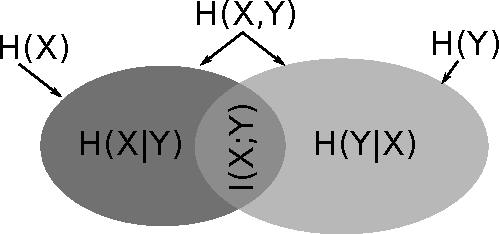
\includegraphics[width=0.75\textwidth]{images/info-set.pdf}
  %\caption{.}
  \label{fig:info-set}
  \end{figure}

\end{frame}

\subsection{Divergência de Kullbach-Leibler}
\begin{frame}%[allowframebreaks]
  \frametitle{Divergência de Kullbach-Leibler}
  A divergência de Kullbach-Leibler é uma relação fundamental entre duas 
  distribuições probabilísticas sobre um mesmo alfabeto, $p=(p_1, \ldots, p_n)$
  e $q=(q_1, \ldots , q_n)$. Esta divergência possui relação importante com a
  entropia e a informação mútua. 

  \vspace{1cm}
  Como podemos medir a `distância' entre duas distribuições $p$ e $q$ de forma útil?
  Poderíamos utilizar $D(p,q) = \sum_{i=1}^n (p_i - q_i)^2$, mas gostaríamos de ter
  uma medida de `distância de informação', isto é, uma distância que nos dê o custo
  incorrido pelo erro de considerar que uma distribuição é $q$ sendo que na realidade
  ela é $p$. Veremos que isto está ligado à insuficiência na compressão. 
  A Divergência de Kullbach-Leibler, definida a seguir, satisfaz estas ideias.
\end{frame}

\begin{frame}[allowframebreaks]
  \frametitle{Distância}
  \begin{definition}[distância]
  Seja $S$ um conjunto. Uma função $d: S \times S \rightarrow \mathbb{R}$ é chamada \textbf{distância} em $S$
  se, para todo $x,y \in S$, tivermos:
  \begin{itemize}
  \item $d(x,y) \geq 0$ (não-negatividade)
  \item $d(x,y) = d(y,x)$ (simetria)
  \item $d(x,x) = 0$ (reflexividade)
  \end{itemize}
  \end{definition}

  \framebreak
  \begin{definition}[métrica]
  Seja $S$ um conjunto. Uma função $d: S \times S \rightarrow \mathbb{R}$ é chamada \textbf{métrica} em $S$
  se, para todo $x,y \in S$, tivermos:
  \begin{itemize}
  \item $d(x,y) \geq 0$ (não-negatividade)
  \item $d(x,y) = 0$ se e somente se $x=y$ (identidade dos indiscerníveis)
  \item $d(x,y) = d(y,x)$ (simetria)
  \item $d(x,y) + d(y,z) \geq d(x,z)$ (desigualdade triangular)
  \end{itemize}
  \end{definition}
\end{frame}
\note{
Teremos uma semi-métrica se substituirmos a identidade dos indiscerníveis pela reflexividade.
}

\begin{frame}%[allowframebreaks]
  \frametitle{Diferentes formas de medir `distância' entre distribuições}

  \begin{description}
  \item[divergência de Kullback-Leibler:] $D_\mathrm{KL}(p \parallel q) = \sum p(x)\ln\left( \frac{p(x)}{q(x)}\right) $;
  \item[distância de Hellinger:] $H^2(p,\, q) = 2 \sum \Big( \sqrt{p(x)} - \sqrt{q(x)}\, \Big)^2 $;
  \item[divergência de Jeffreys:] $D_J(p \parallel q) = \sum (p(x) - q(x))\big( \ln p(x) - \ln q(x) \big) $;
  \item[divergência $\alpha$ de Chernoff:] $D^{(\alpha)}(p \parallel q) = \frac{4}{1-\alpha^2}\bigg(1 - \sum p(x)^\frac{1-\alpha}{2} q(x)^\frac{1+\alpha}{2}  \bigg) $;
  \item[divergência exponencial:] $D_e(p \parallel q) = \sum p(x)\big( \ln p(x) - \ln q(x) \big)^2$;
  \item[divergência de Kagan:] $D_{\chi^2}(p \parallel q) = \frac12 \sum \frac{(p(x) - q(x))^2}{p(x)}$;
  \item[divergência K:] $D_{\mathrm{K}}(p \parallel q) = \sum (p(x) - q(x)) \log(p(x)/q(x))$;
  \item[divergência de Jensen-Shannon:] $D_{\mathrm{JS}}(p \parallel q) = \tfrac{1}{2} D_{\mathrm{KL}} \left (p \parallel m \right ) + \tfrac{1}{2} D_{\mathrm{KL}}\left (q \parallel m \right )\, \!$, onde $m = \tfrac{1}{2}(p+q)$.
  \end{description}
\end{frame}

\begin{frame}%[allowframebreaks]
  \frametitle{Divergência de Kullbach-Leibler (Entropia relativa)}
  Sejam dadas duas distribuições, $p(x)$ e $q(x)$ sobre o mesmo alfabeto,
  $p(x) = P_p (X=x)$ e $q(x) = P_q (X=x)$, a divergência de KL é definida por

  \begin{definition}[Divergência de Kullbach-Leibler (entropia relativa)]
  \begin{equation}
  D(p||q) \triangleq \sum_x p(x) \log \frac{p(x)}{q(x)}
  \end{equation}
  \end{definition}
  Esta divergência pode ser vista como o valor esperado do logaritmo da razão das possibilidades, 
  ponderado por $p$, ou seja, $E_p \log p/q$, ou ainda, o valor esperado da diferença dos 
  logaritmos, $D(p||q) = E_p \left( \log p(x) - \log q(x) \right)$. Fornece a ideia do custo adicional
  (em bits) em se considerar uma distribuição $q$ quando a real distribuição subjacente é $p$.

  Note que a divergência de KL, em geral, não é simétrica, ou seja,
  $D(p||q) \neq D(q||p)$.

\end{frame}
\note{
  Utilizando argumentos de limite e continuidade, mostra-se que $0 \log 0 = 0$
  e $p \log (p/0) = \infty$. Fazendo estas suposições, teremos
  $D(p||q) \leq \infty$.

  A divergência de KL é uma função dos valores de probabilidade e não dos
  valores que a variável aleatória assume (assim como a entropia e a informação mútua).

  \vspace{3em}

A razão de chances ou razão de possibilidades (em inglês: \textit{odds ratio})
é definida como a razão entre a chance de um evento ocorrer em um grupo e a chance de ocorrer em outro grupo.
}
\note{
(Wikipedia)
In statistics, the odds ratio (usually abbreviated "OR") is one of three main ways 
to quantify how strongly the presence or absence of property A is associated with 
the presence or absence of property B in a given population. If each individual in 
a population either does or does not have a property "A", (e.g. "high blood pressure"), 
and also either does or does not have a property "B" (e.g. "moderate alcohol consumption") 
where both properties are appropriately defined, then a ratio can be formed which 
quantitatively describes the association between the presence/absence of "A" 
(high blood pressure) and the presence/absence of "B" (moderate alcohol consumption) 
for individuals in the population. 
}
\note{
This ratio is the odds ratio (OR) and can be computed 
following these steps:
\begin{enumerate}
\item For a given individual that has "B" compute the odds that the same individual has "A"
\item For a given individual that does not have "B" compute the odds that the same individual has "A"
\item Divide the odds from step 1 by the odds from step 2 to obtain the odds ratio (OR).
The term "individual" in this usage does not have to refer to a human being, as 
a statistical population can measure any set of entities, whether living or inanimate.
\end{enumerate}
\url{http://en.wikipedia.org/wiki/Odds_ratio}
}

\begin{frame}%[allowframebreaks]
  \frametitle{Exemplo}
  Seja $\mathcal{X} = \{1,0\}$ e considere duas distribuições $p$ e $q$ em $\mathcal{X}$.
  Seja $p(0)=1-r$, $p(1)=r$, e seja $q(0)=1-s$ e $q(1)=s$. Então
  \begin{equation}
  D(p||q) = (1-r) \log \frac{1-r}{1-s} + r \log \frac{r}{s}
  \end{equation}
  e
  \begin{equation}
  D(q||p) = (1-s) \log \frac{1-s}{1-r} + s \log \frac{s}{r} .
  \end{equation}
  Se $r=s$, então $D(p||q)=D(q||p)=0$. Se $r=\frac{1}{2}$ e $s=\frac{1}{4}$, 
  \begin{equation}
  D(p||q) = \frac{1}{2} \log \frac{1/2}{3/4} + \frac{1}{2} \log \frac{1/2}{1/4} = 1 - \frac{1}{2} \log 3 = 0.2075 \text{bits.}
  \end{equation}
  \begin{equation}
  D(q||p) = \frac{3}{4} \log \frac{3/4}{1/2} + \frac{1}{4} \log \frac{1/4}{1/2} = \frac{3}{4} \log 3 - 1 = 0.1887 \text{bits.}
  \end{equation}

   Note que, em geral, $D(p||q) \neq D(q||p)$.
\end{frame}

\begin{frame}%[allowframebreaks]
  \frametitle{Generalização da divergência de KL}
  A divergência de KL pode ser generalizada para vetores de variáveis aleatórias.

  Seja $p(x_1, \ldots, x_N)$ e $q(x_1, \ldots, x_N)$ duas distribuições sobre o vetor
  $(x_1, x_2, \ldots , x_N)$. A divergência de KL entre $p$ e $q$ é definida por
  \begin{equation}
  D(p||q) = \sum_{x_1, \ldots, x_N} p(x_1, \ldots, x_N) \log \frac{p(x_1, \ldots, x_N)}{q(x_1, \ldots, x_N)}
  \end{equation}
\end{frame}

\begin{frame}[allowframebreaks]
  \frametitle{Divergência de KL e Informação Mútua}
  Seja $\mu_1(x,y) = p(x,y)$ (distribuição conjunta) e $\mu_2(x,y)=p(x)p(y)$ (produto das marginais) 
  com $p(x)=\sum_y p(x,y)$ e $p(y)=\sum_x p(x,y)$, então
  \begin{eqnarray}
  D(\mu_1 || \mu_2) &=& \sum_{x,y} \mu_1(x,y) \log \frac{\mu_1(x,y)}{\mu_2(x,y)} \nonumber \\
                &=& \sum_{x,y} p(x,y) \log \frac{p(x,y)}{p(x)p(y)} = I(X;Y) .
  \end{eqnarray}
  A informação mútua é a distância entre a distribuição conjunta em $X$ e $Y$ e o produto
  das distribuições marginais em $X$ e $Y$.

  Se as v.a.s são independentes, teremos $p(x,y)=p(x)p(y)$ e por conseguinte a divergência será nula,
  a informação mútua entre $X$ e $Y$ será zero.

  A informação mútua é o erro em se assumir independência entre as v.a.s.

  \framebreak
  O produto das distribuições marginais $p(x)p(y)$, onde $p(x)=\sum_y p(x,y)$ e $p(y)=\sum_x p(x,y)$,
  é uma projeção da distribuição conjunta $p(x,y)$ sobre o conjunto das distribuições independentes.
  I.e.,
  \begin{equation}
  p(x)p(y) = \argmin_{p'(x,y) \backslash p'(x,y)=p'(x)p'(y)} D(p(x,y)||p'(x,y)) 
  \end{equation}
\end{frame}


\begin{frame}[allowframebreaks]
  \frametitle{Minimizar a Divergência de KL equivale a maximizar o logaritmo da verossimilhança}
  Suponha que tenhamos uma v.a. $\mathbf{X}=(X_1,\ldots,X_N)$ com uma distribuição subjacente $p$
  que depende de um parâmetro $\theta$ (modelo hipotético). Queremos definir um estimador 
  $\hat{\theta} = T(X_1, \ldots, X_N)$ para este parâmetro $\theta$, dadas as observações $x_1, \ldots, x_N$.
  Um bom estimador para o parâmetro desconhecido $\theta$ é aquela que maximiza a verossimilhança $L(\theta)$ 
  do parâmetro, dada a observação dos dados,
  \begin{equation}
  L(\theta) = \Pr(X_1=x_1, \ldots, X_N=x_N) = p(x_1|\theta) \ldots p(x_N|\theta) = \prod_{n=1}^{N} p(x_n|\theta) .
  \end{equation}
  Como a função logaritmo é monotônica crescente, maximizar $L(\theta)$ é equivalente a maximiza $l(\theta) = \log L(\theta)$,
  \begin{equation} 
  \ell(\theta) = \sum_{n=1}^{N} \log p(x_n|\theta) .
  \end{equation}

  A estimativa de máxima verossimilhança (MLE, \textit{maximum likelihood estimator}) de $\theta$ é dada por
  \begin{equation}
  \hat\theta_\mathrm{mle} = \argmax_{\theta\in\Theta} \ell(\theta\,;\,x_1,\ldots,x_N) .
  \end{equation}

  \framebreak

  Chamaremos de $\hat{p}$ a distribuição empírica. Seja $x_1, \ldots, x_N \in \mathcal{X}$, $N$ observações
  i.i.d. de uma variável aleatória $X$. A distribuição empírica será dada por
  \begin{equation}
  \hat{p}(x) = \frac{1}{N} \sum_{n=1}^{N} \delta(x - x_n) ,
  \end{equation}
  onde $\delta$ é a função de Dirac.

  \vspace{3em}
  Seja $p_\theta$ uma distribuição em $\mathcal{X}$ parametrizada por $\theta$. 
  Maximizar a verossimilhança de $p_\theta(x)$ é equivalente a minimizar a divergência de KL 
  $D_\mathrm{KL}(\hat{p} \parallel p_\theta)$.

  \framebreak

  \begin{eqnarray}
  D_\mathrm{KL}(\hat{p} \parallel p_\theta) &=& \sum_{x \in \mathcal{X}} \hat{p}(x) \log \frac{\hat{p}(x)}{p_\theta(x)} \nonumber \\
        &=& -H(\hat{p}) - \sum_{x \in \mathcal{X}} \hat{p}(x) \log p_\theta(x)  \nonumber \\
        &=& -H(\hat{p}) - \frac{1}{N} \sum_{x \in \mathcal{X}} \sum_{n=1}^{N} \delta(x - x_n) \log p_\theta(x) \nonumber \\
        &=& -H(\hat{p}) - \frac{1}{N} \sum_{n=1}^{N} \log p_\theta(x_n) .
  \end{eqnarray}
  O segundo termo é o oposto do logaritmo da verossimilhança de $p_\theta(x)$.
  
  \framebreak

  A estimativa máxima verossimilhança de $\theta$ a partir das $N$ observações é dada por
  \begin{eqnarray}
  \hat{\theta}_n &=& \argmax_{\theta \in \Theta} \prod_{n=1}^{N} p_\theta(x_n) \nonumber \\
	    &=& \argmax_{\theta \in \Theta} \sum_{n=1}^{N} \log p_\theta(x_n) \nonumber \\
        &=& \argmin_{\theta \in \Theta} \frac{1}{N} \sum_{n=1}^{N} - \log p_\theta(x_n) .
  \end{eqnarray}
   Desta forma, podemos constatar que a distribuição que minimiza a divergência de KL para a distribuição empírica é
   aquela que maximiza a verossimilhança (ou logaritmo desta).
  
%  Pela lei forte dos grandes números, $\frac{1}{N} \sum_{i=1}^{N} \log p_\theta(x_n) \xrightarrow{q.c.} \E[ \log p_\theta(X) ]$.

\end{frame}
% https://www.cs.ubc.ca/~murphyk/Teaching/CS340-Fall06/reading/infoTheory.pdf
% https://www.di.ens.fr/~fbach/courses/fall2013/lecture5.pdf
% http://nowak.ece.wisc.edu/SLT09/lecture13.pdf


\subsection{Informação Mútua Condicional}
\begin{frame}%[allowframebreaks]
  \frametitle{Informação Mútua Condicionada a um evento}
  A informação pode se alterar se for condicionada a um evento de uma terceira variável
  aleatória $\{Z=z\}$, e isto é denotado por $I(X;Y|Z=z)$, onde $X,Y,Z$ são variáveis
  aleatórias.

  Dada a distribuição $p(x,y,z)$, a informação mútua condicionada ao evento específico
  $\{Z=z\}$ é dada por
  \begin{equation}
  I(X;Y|Z=z) = \sum_{x,y} p(x,y|z) \log \frac{p(x,y|z)}{p(x|z)p(y|z)} .
  \end{equation}

  Obs. Fazemos as seguintes alterações sobre a informação mútua padrão: 
  $p(x,y)\rightarrow p(x,y|z)$, $p(x)\rightarrow p(x|z)$ e $p(y) \rightarrow p(y|z)$.
\end{frame}

\begin{frame}%[allowframebreaks]
  \frametitle{Informação Mútua Condicional}
   A informação entre duas variáveis aleatórias pode mudar na média se for condicionada 
   a uma terceira variável aleatória. Será denotada por $I(X;Y|Z)$.
   \begin{definition}[Informação Mútua Condicional]
   \vspace{-0.3cm}
   \begin{eqnarray}
     I(X;Y|Z) &\triangleq& \sum_z p(z) I(X;Y|Z=z) \nonumber \\
                &=& \sum_z p(z) E_{p(x,y|z)} \log \frac{p(x,y|Z=z)}{p(x|Z=z) p(y|Z=z)} \nonumber \\
                &=& \sum_{x,y,z} p(x,y,z) \log \frac{p(x,y|z)}{p(x|z)p(y|z)} \nonumber \\
                &=& E \left[ \log \frac{1}{p(x|z)} - \log \frac{1}{p(x|y,z)} \right] \nonumber \\
                &=& H(X|Z) - H(X|Y,Z)
   \end{eqnarray}
   \end{definition}
\end{frame}
\note{
\begin{equation}
 I(X;Y) = H(X) - H(X|Y)
\end{equation}

\begin{equation}
 I(X;Y|Z) = H(X|Z) - H(X|Y,Z)
\end{equation}
}



\subsection{Propriedades da Informação Mútua}
\begin{frame}%[allowframebreaks]
  \frametitle{Regra da Cadeia para Informação Mútua}
   \begin{proposition} \vspace{-0.2cm}
   \begin{equation}
   I(X_1,X_2,\ldots,X_N;Y) = \sum_i I(X_i;Y|X_1,X_2,\ldots,X_{i-1})
   \end{equation}
   \end{proposition}
   
   Exemplo: $I(X_1,X_2;Y) = I(X_1;Y) + I(X_2;Y|X_1)$
   \begin{proof} \vspace{-0.6cm}
   \begin{eqnarray}
        I(X_1,\ldots,X_N;Y) &=& H(X_1,\ldots,X_N) - H(X_1,\ldots,X_N|Y) \nonumber \\
                &=& \sum_{i=1}^N H(X_i|X_1,\ldots,X_{i-1}) - \sum_{i=1}^N H(X_i|X_1,\ldots,X_{i-1},Y) \nonumber \\
                &=& \sum_{i=1}^N I(X_i;Y|X_1,\ldots,X_{i-1}) 
   \end{eqnarray}
   \end{proof}
\end{frame}

\begin{frame}%[allowframebreaks]
  \frametitle{Entropia Relativa Condicional - divergência de KL}
  \begin{definition}
  Para pmf conjuntas $p(x,y)$ e $q(x,y)$, a entropia relativa condicional é definida como
  \begin{eqnarray}
        D(p(y|x) || q(y|x)) &\triangleq& \sum_x p(x) \sum_y p(y|x) \log \frac{p(y|x)}{q(y|x)} \nonumber \\
                &=& \sum_{x,y} p(x,y) \log \frac{p(y|x)}{q(y|x)} \nonumber \\
                &=& \E_{p(x,y)} \log \frac{p(Y|X)}{q(Y|X)} ,
  \end{eqnarray}
  é o valor esperado das entropias relativas entre as pmfs condicionais $p(y|x)$ e $q(y|x)$, 
  tomando o valor esperado sobre a distribuição de massa $p(x)$.
  \end{definition} 
\end{frame}


\begin{frame}%[allowframebreaks]
  \frametitle{Regra da Cadeia para divergência de KL}
  \begin{proposition}
  \begin{equation}
  D(p(x,y)||q(x,y)) = D(p(x)||q(x)) + D(p(y|x)||q(y|x))
  \end{equation}
  \end{proposition}

  \begin{proof}
  \begin{eqnarray}
  D(p(x,y)||q(x,y)) &=& \sum_{x,y} p(x,y) \log \frac{p(x,y)}{q(x,y)} = \sum_{x,y} p(x,y) \log \frac{ p(y|x)p(x) }{ q(y|x)q(x) } \nonumber \\
        &=& \sum_{x,y} p(x,y) \log \frac{ p(y|x) }{ q(y|x) } + \sum_{x,y} p(x,y) \log \frac{ p(x) }{ q(x) } 
  \end{eqnarray}
  \end{proof}
\end{frame}



\subsection{Desigualdade de Jensen}
\begin{frame}%[allowframebreaks]
  \frametitle{Funções Convexas}
   \begin{definition}
   Dizemos que $f$ é convexa em $(a,b)$ se para todo $x_1,x_2 \in (a,b)$, $0 \leq \lambda \leq 1$,
   \begin{equation}
   f(\lambda x_1 + (1 - \lambda)x_2) \leq \lambda f(x_1) + (1-\lambda) f(x_2)
   \end{equation}
   \end{definition}
   Exemplos:  
    \begin{inlineenumerate}
        \item $f(x)=x^2$
        \item $f(x)=e^x$
        \item $x \log x$, $x \geq 0$.
    \end{inlineenumerate}
  \begin{figure}[h!]
  \centering
  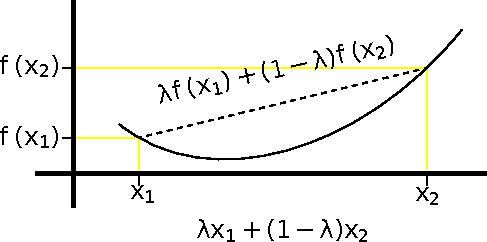
\includegraphics[width=0.5\textwidth]{images/funcao-convexa.pdf}
  %\caption{.}
  \label{fig:funcao-convexa}
  \end{figure}
  \begin{itemize}
  \item $f$ é estritamente convexa se a igualdade for verdadeira 
  apenas para $\lambda = 0$ ou $\lambda = 1$.
  \end{itemize}
\end{frame}

\begin{frame}[allowframebreaks]
  \frametitle{Derivada Segunda e Convexidade}
  \begin{theorem}[derivada segunda e convexidade]
  Se uma função $f$ possui derivada segunda não-negativa (positiva) em um intervalo,
  a função é convexa (estritamente convexa) no intervalo.
  \end{theorem}

  \begin{proof}
  A expansão de Taylor de uma função $f$ em torno do ponto $x_0$ é dada por
  \begin{equation}
  f(x) = f(x_0) + f'(x_0) (x-x_0) + \frac{f''(x^\ast)}{2} (x-x_0)^2
  \end{equation}
  onde $x^\ast \in (x_0,x)$. Por hipótese, $f''(x^\ast) \geq 0$, e desta forma,
  o último termo é não-negativo.

  \proofbreak

  Seja $x_0 = \lambda x_1 + (1-\lambda) x_2$. Analisando em $x=x_1$, teremos
  \begin{eqnarray}
    f(x_1) &\geq& f(x_0) + f'(x_0) (x_1 - \lambda x_1 - (1-\lambda)x_2) \nonumber \\
        &=& f(x_0) + f'(x_0) ((1-\lambda)(x_1-x_2)) \label{eq-274}
  \end{eqnarray}
  Da mesma forma, em $x=x_2$, teremos
  \begin{eqnarray}
    f(x_2) &\geq& f(x_0) + f'(x_0) (x_2 - \lambda x_1 - (1-\lambda)x_2) \nonumber \\
        &=& f(x_0) + f'(x_0) (\lambda(x_2-x_1)) \label{eq-275}
  \end{eqnarray}

  \proofbreak

  Somando $\lambda$ \ref{eq-274} com $(1-\lambda)$ \ref{eq-275}, teremos
  \begin{eqnarray}
  \lambda f(x_1) + (1-\lambda) f(x_2) &\geq& \lambda f(x_0) + \lambda f'(x_0) ((1-\lambda)(x_1-x_2)) + \nonumber \\
                        && (1-\lambda) f(x_0) + (1-\lambda) f'(x_0) (\lambda(x_2-x_1)) \nonumber \\
        &\geq& f(x_0) = f(\lambda x_1 + (1-\lambda) x_2)
  \end{eqnarray}

  \end{proof} 
\end{frame}

\begin{frame}%[allowframebreaks]
  \frametitle{Desigualdade de Jensen}
  \begin{theorem}[Jensen]
  Seja $f$ uma função convexa e $X$ uma variável aleatória, então
  \begin{equation}
    E f(X) = \sum_x p(x) f(x) \geq f(E X) = f \left( \sum_x x p(x) \right)
  \end{equation}
  \end{theorem}

  Se $f$ é estritamente convexa, então $\{E f(X) = f(E(X))\} \Rightarrow \{X = EX\}$,
  o que significa que $X$ é uma v.a. constante.
\end{frame}

\begin{frame}[allowframebreaks]
  \frametitle{Desigualdade de Jensen - demonstração}
  \begin{itemize}
   \item Para uma distribuição de massa com apenas dois pontos.
   \begin{equation}
    E[f(X)] = p_1 f(x_1) + p_2 f(x_2) \geq f(p_1 x_1 + p_2 x_2) = f(EX)
   \end{equation} 
   já que $f$ é convexa e $p_1+p_2=1$.
   \item Para uma distribuição com mais de dois ponto, iremos fazer uma demonstração 
   por indução.
  \end{itemize}

  \begin{proof}
  Suponha que o teorema seja verdadeiro para uma distribuição com $k-1$ pontos de massa.
  Para uma distribuição com $k$ pontos de massa podemos escrever cada 
  $p_i' = p_i / (1-p_k)$ para $i=1,2,\ldots,k-1$. 
  \proofbreak
  Desta forma, teremos
  \begin{eqnarray}
   E[f(X)] &=& \sum_{i=1}^k p_i f(x_i) \nonumber \\
        &=& \sum_{i=1}^{k-1} (1-p_k)p_i' f(x_i) + p_k f(x_k) \nonumber \\
        &=& (1-p_k) \sum_{i=1}^{k-1} p_i' f(x_i) + p_k f(x_k) \nonumber 
   \end{eqnarray}

   \proofbreak

   Poderemos utilizar a hipótese de indução, já que
   \begin{equation}
   \sum_{i=1}^{k-1} p_i' = \sum_{i=1}^{k-1} \frac{p_i}{1-p_k} = \frac{1-p_k}{1-p_k} = 1 .
   \end{equation}
   Então
   \begin{eqnarray}
   E[f(X)] &=& \ldots \nonumber \\
        &\geq& (1-p_k) f\left( \sum_{i=1}^{k-1} p_i' x_i \right) + p_k f(x_k) \nonumber
   \end{eqnarray}
  
   \proofbreak

   Pela definição de convexidade, teremos
   \begin{eqnarray}
   E[f(X)] &=& \ldots \nonumber \\
        &\geq& f \left( (1-p_k) \sum_{i=1}^{k-1} p_i' x_i + p_k x_k \right) \nonumber \\ 
        &=& f\left( \sum_{i=1}^{k} p_i x_i \right)
   \end{eqnarray}

   Desta forma, sendo o teorema válido para uma distribuição de massa com $k-1$ pontos,
   também será verdadeiro para uma distribuição de massa com $k$ pontos.
   Como mostramos que para $k=2$ é verdadeiro, logo o teorema é verdadeiro para qualquer $k$.
  \end{proof}
\end{frame}

\begin{frame}%[allowframebreaks]
  \frametitle{Desigualdade de Jensen - demonstração gráfica}

  \vspace{-0.2cm}
  \begin{figure}[h!]
  \centering
  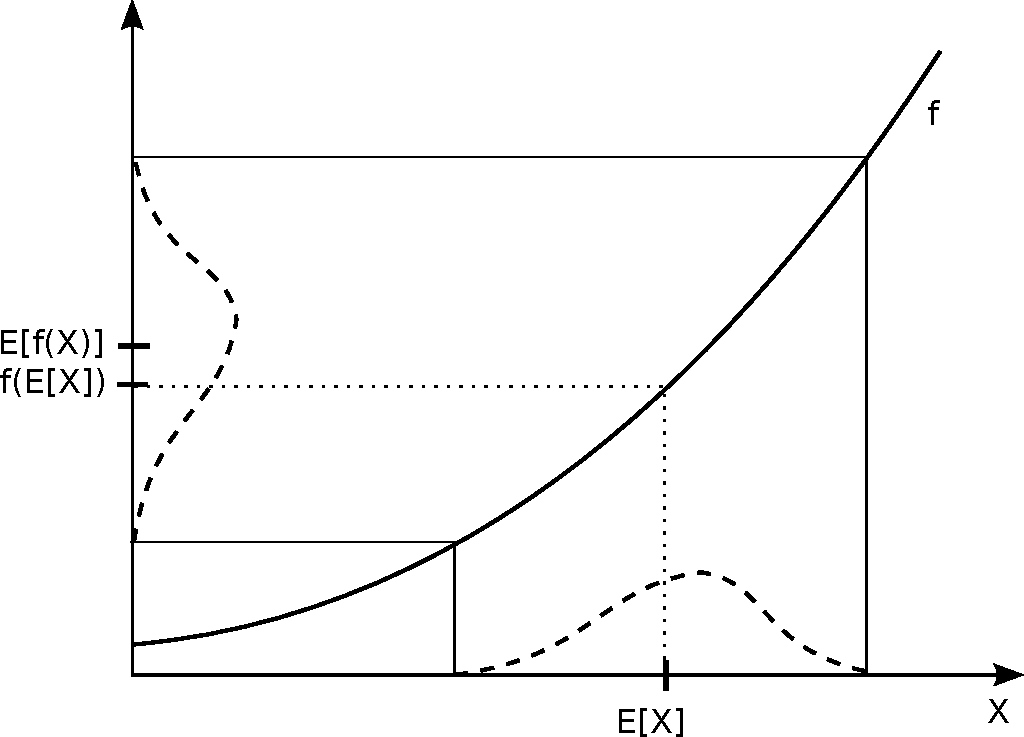
\includegraphics[width=0.5\textwidth]{images/jensen.pdf}
  %\caption{.}
  \label{fig:jensen}
  \end{figure} 

  \vspace{-0.2cm}
  O mapeamento feito pela função convexa $f$ aumenta gradativamente o estiramento
  da distribuição mapeada por $f$ com o aumento dos valores de $X$.
  Desta forma, o valor esperado da distribuição mapeada por $f$ tende a possuir
  um valor maior que o mapeamento por $f$ do valor esperado da distribuição.
\end{frame}


\subsection{Não-Negatividade}
\begin{frame}%[allowframebreaks]
  \frametitle{A divergência de KL é não-negativa}
  \begin{lemma} 
  \begin{equation}
  D(p||q) \geq 0 \text{ com igualdade se e somente se } p(x) = q(x) \forall x.
  \end{equation}
  \end{lemma}
\end{frame}

\begin{frame}%[allowframebreaks]
  \frametitle{A divergência de KL é não-negativa} 
  \begin{proof}
  Mostre que $-D(p||q) \leq 0$. Seja $S_p=\{x: p(x) > 0\} = \sup (p)$, então
  \begin{eqnarray}
  -D(p||q) &=& -\sum_x p(x) \log \frac{p(x)}{q(x)} = -\sum_{x \in S_p} p(x) \log \frac{p(x)}{q(x)} %\nonumber \\
        = \sum_{x \in S_p} p(x) \log \frac{q(x)}{p(x)} = E \log \frac{q(X)}{p(X)} \nonumber \\
        && {\small \text{utilizando a desigualdade de Jensen}} \nonumber \\
        &\leq& \log \left( E \frac{q(X)}{p(X)} \right) = \log \left( \sum_{x \in S_p} p(x) \frac{q(x)}{p(x)} \right) \nonumber \\
        &=& \log \left( \sum_{x \in S_p} q(x) \right) \leq \log \left( \sum_x  q(x) \right) = \log 1 = 0
  \end{eqnarray}
  \end{proof}
\end{frame}

\begin{frame}%[allowframebreaks]
  \frametitle{A divergência de KL é não-negativa}
  \begin{itemize}
  \item Note que $\log x$ é estritamente côncavo.
  \item Então, a igualdade $\sum_{x \in S_p} p(x) \frac{q(x)}{p(x)} = \log \left( \sum_{x \in S_p} p(x) \frac{q(x)}{p(x)} \right)$ significa $Z=E Z$ com $Z = q(X)/p(X)$, então $Z$ é uma variável aleatória constante.
  \item A única constante válida, com $p$ e $q$ sendo distribuições de probabilidade é
  $Z=1$ ou $p(x)=q(x)$.
  \item Então, se $p(x)=q(x)$ teremos $D(p||q)=0$ e vice-versa.
  \end{itemize}
\end{frame}

\begin{frame}%[allowframebreaks]
  \frametitle{A informação mútua é não-negativa}
  \begin{proposition}
  \begin{equation} 
  I(X;Y) \geq 0 \text{ e } I(X;Y) = 0 \Leftrightarrow X \independent Y.
  \end{equation}
  \end{proposition}

  \begin{proof}
  \begin{equation}
  I(X;Y) = D(p(x,y)||p(x)p(y)) \geq 0
  \end{equation}
  \end{proof}
  teremos igualdade se $p(x,y)=p(x)p(y)$, o que é também condição para independência.
\end{frame}

\begin{frame}%[allowframebreaks]
  \frametitle{Informação Mútua}
  \begin{itemize}
  \item $I(X;Y)$ mede o `grau de dependência' entre $X$ e $Y$.
  \item Temos $0 \leq I(X;Y) \leq \min (H(X),H(Y))$.
  \item $I(X;Y) = H(X) - H(X|Y) = H(Y) - H(Y|X)$.
  \item Se $X \independent Y$, então $I(X;Y)=0$, já que em tal caso $H(X|Y)=H(X)$
  e $H(Y|X)=H(Y)$.
  \item Se $X=Y$, então $I(X;Y) = H(X) = H(Y)$ já que em tal caso $H(Y|X)=H(X|Y)=0$.
  \end{itemize}
\end{frame}


\subsection{Limite Superior para a Entropia}
\begin{frame}[allowframebreaks]
  \frametitle{Limite Superior para a Entropia}
  \begin{theorem}
  $H(X) \leq \log \vert \mathcal{X} \vert$, onde $\vert \mathcal{X} \vert$ denota
  o número de elementos da extensão de $X$ (a cardinalidade do domínio), com igualdade
  se e somente se $X$ possuir distribuição uniforme.
  \end{theorem}

  \framebreak

  \begin{proof}
  Seja $u(x) = \frac{1}{\vert \mathcal{X} \vert}$ a função probabilidade de massa uniforme
  em $\mathcal{X}$, e seja $p(x)$ a função probabilidade de massa para $X$. Então
  \begin{eqnarray}
  D(p||u) &=& \sum_{x \in \mathcal{X}} p(x) \log \frac{p(x)}{u(x)} \nonumber \\
        &=& \sum_{x \in \mathcal{X}} p(x) \log p(x) + \sum_{x \in \mathcal{X}} p(x) \log \frac{1}{u(x)} \nonumber \\
        &=& -H(X) + \log \vert \mathcal{X} \vert \sum_{x \in \mathcal{X}} p(x) \nonumber \\
        &=& \log \vert \mathcal{X} \vert - H(X)
  \end{eqnarray}
  \proofbreak
  Como a entropia relativa é não negativa, $D(p||u) \geq 0$, teremos
  \begin{equation}
  D(p||u) = \log \vert \mathcal{X} \vert - H(X) \geq 0
  \end{equation}
  e assim
  \begin{equation}
  H(X) \leq \log \vert \mathcal{X} \vert
  \end{equation}
  \end{proof}
\end{frame}


\subsection{Condicionar Reduz Entropia}
\begin{frame}%[allowframebreaks]
  \frametitle{Condicionar Reduz Entropia}
  Comparando $H(X)$ com $H(X|Y)$, conhecendo $Y$, na média, pode nos dizer algo sobre $X$
  reduzindo a entropia.
  \begin{proposition}
  \begin{equation}
  H(X|Y) \leq H(X) \text{ e } H(X|Y) = H(X) \text{ se e somente se } X \independent Y.
  \end{equation}
  \end{proposition}

  \begin{proof}
  \begin{equation}
  0 \leq I(X;Y) = H(X) - H(X|Y)
  \end{equation}
  \end{proof}

  Poderíamos ter $H(X|Y=y) > H(X)$, mas, na média, $\sum_y p(y) H(X|Y=y) \leq H(X)$.
\end{frame}


\begin{frame}%[allowframebreaks]
  \frametitle{Limite da Entropia para um Conjunto de V.A.}
  A entropia de um conjunto de variáveis aleatórias é maior quando as
  variáveis aleatórias são independentes, há menor redundância entre elas.
  \begin{proposition}\label{prop-lim-ent-conj-va}
  \begin{equation}\label{eq-lim-ent-conj-va}
  H(X_1, X_2, \ldots, X_N) \leq \sum_{i=1}^N H(X_i)
  \end{equation}
  \end{proposition}

  \begin{proof}
  \begin{equation}
  H(X_1, \ldots, X_N) = \sum_{i=1}^N H(X_i | X_1, \ldots, X_{i-1}) \leq \sum_{i=1}^N H(X_i)
  \end{equation}
  \end{proof}

\end{frame}
\note{
 \begin{equation}
 \sum_{i=1}^N H(X_i | X_{\neg i}) = \sum_{i=1}^N H(X_i | X_1, \ldots, X_{i-1}, X_{i+1}, \ldots, X_N) \leq H(X_1, \ldots, X_N)
 \end{equation}
}

\begin{frame}%[allowframebreaks]
  \frametitle{Limites da Independência na Entropia}
  A proposição \ref{prop-lim-ent-conj-va} para duas variáveis é da forma
  \begin{equation}
  H(X_1,X_2) \leq H(X_1) + H(X_2)
  \end{equation}
  Note que a igualdade na Equação \ref{eq-lim-ent-conj-va} é alcançada quando
  todas as variáveis são mutuamente independentes, isto é, quando $X_i \independent X_j \forall i,j$.
\end{frame}


\begin{frame}%[allowframebreaks]
  \frametitle{Condicionamento e Informação Mútua}
  \begin{itemize}
  \item Se $X \independent Y|Z$ então $I(X;Y|Z)=0$. Por exemplo, $X \independent Y|Z$ quando
  $X \rightarrow Z \rightarrow Y$.
  \item Alternativamente, se $Z=Y$, então $I(X;Y|Z)=0$.
  \item Podemos ter $I(X;Y) > I(X;Y|Z)$.
  \item Por outro lado, se $Z=X+Y$ e $X \independent Y$, então $I(X;Y)=0$ mas 
  $I(X;Y|Z)>0$.
  \item Não existe uma relação genérica entre informação mútua e informação mútua condicional.
  \end{itemize}
\end{frame}

\begin{frame}%[allowframebreaks]
  \frametitle{Relações de H}

  \begin{equation}
  H(X) = E I(X) = - \sum_x p(x) \log p(x)
  \end{equation}

  \begin{equation}
  H(X,Y) = - \sum_{x,y} p(x,y) \log p(x,y)
  \end{equation}

  \begin{equation}
  H(Y|X) = - \sum_{x,y} p(x,y) \log p(y|x)
  \end{equation}

  \begin{equation}
  H(X,Y) = H(X) + H(Y|X) = H(Y) + H(X|Y)
  \end{equation}

  \begin{equation}
  I(X;Y) = H(X) - H(X|Y) = H(Y) - H(Y|X)
  \end{equation}

  \begin{equation}
  0 \leq H(X) \leq \log n, \text{ onde } n \text{ é o tamanho do alfabeto de } X.
  \end{equation}
\end{frame}

\begin{frame}%[allowframebreaks]
  \frametitle{Entropia, Informação Mútua, 3 V.A. em um diagrama de Venn}
  \begin{figure}[h!]
  \centering
  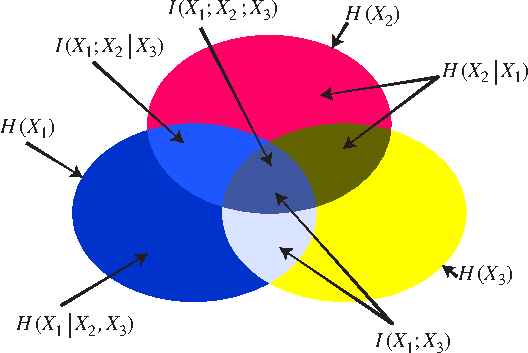
\includegraphics[width=0.7\textwidth]{images/3va-venn.pdf}
  %\caption{.}
  \label{fig:3va-venn}
  \end{figure}
\end{frame}
\note{
\begin{itemize}
 \item $I(X_1;X_2) = I(X_1;X_2|X_3) + I(X_1;X_2;X_3)$.
 \item $I(X_1;X_2) \gtreqqless I(X_1;X_2|X_3)$, mas isto nunca será negativo. 
 \item Então, $I(X_1;X_2;X_3) = I(X_1;X_2) - I(X_1;X_2|X_3)$ pode ser negativo.
 \item $I(X_1;X_2;X_3) = I(X_1;X_2) - I(X_1;X_2|X_3) = I(X_2;X_3) - I(X_2;X_2|X_1) = I(X_3;X_1) - I(X_3;X_1|X_2)$
 \item $I(X_1;X_2;X_3) = H(X_1) + H(X_2) + H(X_3) - H(X_1;X_2) - H(X_2;X_3) - H(X_3;X_1) + H(X_1,X_2,X_3)$
\end{itemize}
}


\begin{frame}[allowframebreaks]
  \frametitle{Revisão}
  \begin{itemize}
  \item divergência de KL: $D(p||q) = \sum_x p(x) \log \frac{p(x)}{q(x)}$
  \item informação mútua: $I(X;Y) = \sum_{x,y} p(x,y) \log \frac{p(x,y)}{p(x)p(y)} = D(p(x,y)||p(x)p(y))$ 
  \item informação mútua condicional: $I(X;Y|Z) = \sum_{x,y,z} p(x,y,z) \log \frac{p(x,y|z)}{p(x|z) p(y|z)} = H(X|Z) - H(X|Y,Z)$
  \item regra da cadeia da informação mútua: $I(X_1,X_2,\ldots,X_N;Y)=\sum_i I(X_i;Y|X_1,X_2,\ldots,X_{i-1})$
  \item entropia relativa condicional: $D(p(y|x)||q(y|x)) \triangleq \sum_{x,y} p(x,y) \log \frac{p(y|x)}{q(y|x)}$
  \item regra da cadeia da divergência de KL: $D(p(x,y)||q(x,y)) = D(p(x)||q(x)) + D(p(y|x)||q(y|x))$
  \item Jensen: $f$ convexa $\Rightarrow$ $E f(X) = \sum_x p(x) f(x) \geq f(E X) = f \left( \sum_x p x(x) \right)$
  \item não negatividade da divergência de KL: $D(p||q) \geq 0$, $D(p||q)=0 \Leftrightarrow p=q$.
  \item não negatividade da informação mútua: $I(X;Y)\geq 0$, $I(X;Y)=0 \Leftrightarrow X \independent Y$.
  \item condicionar reduz a entropia: $H(X) \geq H(X|Y)$, $H(X) = H(X|Y) \Leftrightarrow X \independent Y$.
  \item limite da independência em H: $H(X_1,\ldots,X_N) \leq \sum_{i} H(X_i)$, com igualdade sse todos $X_i$ forem independentes
  \end{itemize}
\end{frame}


